\chapter{Implementacja}

Głównym założeniem projektu było stworzenie go w taki sposób, aby kod jak najtrafniej odzwierciedlał rzeczywistość. W tym celu stworzono klasy obiektów reprezentujące rzeczywiste byty w świecie realnym.
\begin{figure}[H]
\centering
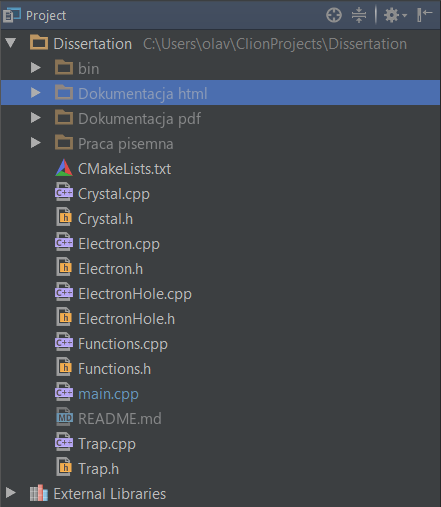
\includegraphics[width=15cm]{strukturaprojektu}
\caption{Struktura projektu.}
\label{fig:Struktura projektu}
\end{figure}

\section{Kod}
\subsection{Konwencja nazw}
W czasie tworzenia projektu kierowano się standardowym, spójnym stylem nazywania klas, metod i zmiennych.
 
Nazwy klas zaczynają się z wielkiej litery, jeśli nazwa zawiera więcej niż jedno słowo to każde z nich zaczyna się wielką literą np. \textit{ElectronHole}. 

Nazwy zmiennych oraz metod zaczynają się z małej litery. Jeśli nazwy złożone są z wielu słów, każde kolejne słowo poza pierwszym zaczyna się z wielkiej litery np. \textit{tunnelEffectProbability(double time, double tau)}. 

Argumenty funkcji zaczynają się z małej litery. W przypadku użycia argumentu składającego się z wielu wyrazów oddzielane są one znakiem '\_'  np. \textit{Crystal(long long int n\_el, long long n\_holes, double min, double max)}.

\subsection{Formatowanie i dokumentacja}

W projekcie użyto spójnego stylu "wcinania" kodu za pomocą funkcji \textbf{Reformat Code} programu CLion (skrót Ctrl + Alt + L). Dzięki temu kod stał się dużo bardziej przejrzysty dla programisty.

Każda z klas została umieszczona w osobnych plikach .cpp oraz .h . W plikach .h znajduje się deklaracja klasy wraz z jej metodami i zmiennymi. W plikach .cpp zostały umieszczone implementacje metod dla odpowiednich klas. 

Aby kod był łatwiejszy do zrozumienia oraz rozwijania, w folderze \href{www}{Dokumentacja} znajduje się dokumentacja projektu wykonana za pomocą programu \textbf{doxygen}. Zawiera ona informacje na temat metod i składowych wszystkich wykorzystywanych klas.

\section{Klasy}
Każda z klas posiada własne metody w zależności od swojego przeznaczenia.

Klasa \textit{Electron} odzwierciedla cząstkę elementarną - elektron. Zmiana ilości tych cząstek w stanie wzbudzonym tj. znajdujących się w pułapce jest głównym celem wykonania tej symulacji.

\textit{ElectronHole} jest reprezentacją dziury elektronowej, z którą to elektron po wykorzystaniu zjawiska tunelowego zrekombinuje. Głównymi składowymi tej klasy są: wektor pozycji dziury, wskaźnik na obiekt typu \textit{Trap} oraz energia dziury wyrażona w elektronowolotach. 

Klasa \textit{Trap} odpowiada defektom w sieci krystalicznej czyli pułapkom, które mogą przechwycić elektron lub dziurę elektronową. Posiada metodę \textit{isOccupied()}, która jest warunkiem sprawdzanym za każdym razem gdy symulowany jest efekt tunelowy. Na potrzeby wykonania tej symulacji założono, że na samym jej początku wszystkie obiekty reprezentujące elektrony oraz dziury elektronowe znajdują się już w pułapkach. Oznacza to, że konstruktor tej klasy ustawia wskaźnik \textit{electron} na podany obiekt typu \textit{Electron}. Dodatkowo, w symulacji ustalono, że dany elektron jeśli spełni warunek wystąpienia zjawiska tunelowego - po jego zajściu i rekombinacji z dziurą - nie może przetunelować ponownie. Zostało to podyktowane zmniejszeniem oczekiwanego czasu działania programu.

Klasa \textit{Crystal} reprezentuje rzeczywisty kryształ, który będzie poddany symulacji zaniku sygnału luminescencyjnego. Zawiera on w sobie inne obiekty takie jak:

\begin{itemize}
\item Elektrony
\item Dziury elektronowe
\item Obiekty odpowiadające defektom sieci krystalicznej - tzw. pułapki
\end{itemize}

Jest to główna klasa zarządzająca całą symulacją. Posiada metody wyliczające niezbędne parametry równania \ref{eq:1}, a także zapisujące wynik działania programu do pliku w odpowiednich jednostkach.





\section{Opis działania programu}



W celu otrzymania danych niezbędnych do wygenerowania wykresu zależności między ilością elektronów w pułapkach a upływem czasu uruchomiono stworzony program. Obiekt \textit{Crystal} w swoim konstruktorze generuje podaną ilość dziur elektronowych, pułapek oraz elektronów, a następnie przechowuje je w oddzielnych kontenerach. Dla każdej z tych cząstek wywoływany jest konstruktor (ustawiający współrzędne położenia) z argumentami, które są losowane z podanego wcześniej przedziału (wartości są podane w Angstremach tj. 1 Å = $10^{-10}$m). Jednostka ta nie jest jednostką układu SI, lecz jest stosowana w fizyce przy opisywaniu obiektów i zjawisk zachodzących w skali atomowej). Jak podkreślono wcześniej, symulacja zakłada, że na jej starcie każdy elektron znajduje się w pułapce. Powoduje to, że para elektron - pułapka ma identyczne współrzędne położenia, a także obiekt klasy \textit{Trap} przyjmuje wskaźnik na uwięziony w nim elektron.

Następnie za pomocą metody \textit{startSimulation(int time)} obiektu klasy \textit{Crystal} rozpoczyna symulację. Symulowany upływ czasu  zależy od wartości argumentu \textit{time}, który jest wyrażony w dniach tj. wywołanie \emph{startSimulation(365)} oznacza rozpoczęcie działania symulacji symulującej efekt zaniku sygnału luminescencyjnego w czasie 1 roku.

Podczas wykonywania symulacji każda pułapka elektronowa jest sprawdzana czy przechowuje w sobie uwięziony elektron. Jeśli warunek jest spełniony, to dla elektronu oraz dziur elektronowych znajdujących się w pułapkach, za pomocą wzoru \ref{eq:1} wyliczane jest prawdopodobieństwo zajścia efektu tunelowego. Jeśli prawdopodobieństwo jest mniejsze ( ponieważ wzór \ref{eq:1} oblicza prawdopodobieństwo, że tunelowanie nie zajdzie) od losowej liczny z zakresu [0,1] to elektron opuszcza swoją pułapkę (wskaźnik obiektu klasy \textit{Trap} na elektron ustawiany jest na wartość \textit{NULL}), a następnie zmienia swoje dotychczasowe położenie na współrzędne do których przetunelował (współrzędne centrum rekombinacyjnego/dziury). Powtarzane jest to tak długo, aż program za symuluje podany mu wcześniej czas trwania symulacji.  Jak wynika z założeń projektu wspomnianych wcześniej - jeśli elektron przetunelował do centrum rekombinacji przynajmniej raz, nie będzie on brał więcej udziału w obliczaniu prawdopodobieństwa zajścia efektu tunelowego. 

Po skończeniu symulacji, program zapisuje do pliku tekstowego otrzymane wyniki w formacie \textit{czas;ilość elektronów w stanie wzbudzenia}, gdzie czas wyrażony jest w $ \log(\frac{t}{2 dni}) $, a ilość elektronów oznacza jaka część z początkowych elektronów nadal znajduje się w pułapkach. Za pomocą skryptu \textit{wykres.plt}
w folderze \href{www}{\textit{bin/Debug}} generowany jest odpowiedni wykres ilustrujący otrzymane dane. 

Przykładowo wygenerowany wykres (analiza otrzymanych wykresów znajduje się w dalszej części pracy):

\begin{figure}[H]
\centering
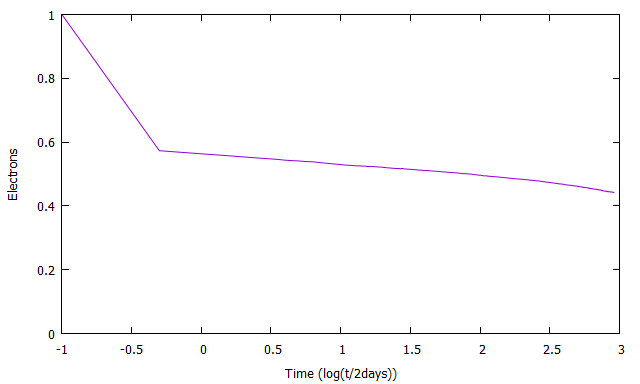
\includegraphics[width=15cm]{example}
\caption{Przykładowa wizualizacja otrzymanych danych}
\label{fig:example}
\end{figure}

